\subsection{Hiện thực hóa và triển khai backend}

\subsubsection{Hiện thực hóa các mã nguồn backend}

\textbf{Kiến trúc phân lớp và điều phối luồng dữ liệu}

Tất cả các dịch vụ trong hệ thống được xây dựng trên một cấu trúc đồng nhất, áp dụng mô hình CQRS để tách biệt hoàn toàn luồng xử lý ghi dữ liệu và luồng truy vấn dữ liệu. Cấu trúc này giúp tối ưu hóa hiệu năng và tăng khả năng bảo trì hệ thống.

\begin{itemize}
    \item Nhóm Commands: Tập trung vào việc xử lý các yêu cầu thay đổi trạng thái như tạo mới, cập nhật hoặc xóa. Luồng đi từ Controller qua Service Interface đến Service thực thi và được hỗ trợ bởi các Event Handler để xử lý các sự kiện bất đồng bộ liên quan đến Kafka.
    \item Nhóm Queries: Chuyên biệt cho các tác vụ lấy dữ liệu. Luồng này được tối ưu để trả về kết quả nhanh nhất mà không cần đi qua các bước kiểm tra nghiệp vụ phức tạp của luồng ghi.
\end{itemize}

\textbf{Tổ chức đối tượng truyền tải dữ liệu DTO}

Dữ liệu trao đổi giữa client và server hoặc giữa các dịch vụ với nhau được chuẩn hóa trong thư mục dto. Các lớp này được phân chia chi tiết thành Requests và Responses cho từng loại nghiệp vụ cụ thể như auth, address, hay payment\_account. Việc tách bạch DTO cho Command và Query đảm bảo tính chặt chẽ của dữ liệu đầu vào và đầu ra, tránh việc phơi bày các thực thể cơ sở dữ liệu trực tiếp ra bên ngoài.

\textbf{Tầng truy xuất dữ liệu Repository}

Tương ứng với mô hình CQRS, tầng Repository được chia làm hai loại:

\begin{itemize}
    \item jpa\_repositories: Sử dụng Spring Data JPA để thực hiện các thao tác lưu trữ và cập nhật vào cơ sở dữ liệu.
    \item read\_only\_repositories: Được cấu hình tối ưu chỉ để đọc dữ liệu, giúp giảm tải cho hệ thống và tăng tốc độ phản hồi cho các yêu cầu truy vấn.
\end{itemize}

\textbf{Các thành phần hỗ trợ hệ thống}

\begin{itemize}
    \item Mapper và Factory: Tầng mapper chịu trách nhiệm chuyển đổi dữ liệu giữa Model và DTO một cách tự động. Tầng factory được sử dụng để khởi tạo các đối tượng phức tạp, đảm bảo tính đóng gói của mã nguồn.
    \item Email Handler và Util: Các tác vụ bổ trợ như gửi email thông báo được tách thành module riêng để không gây nghẽn luồng xử lý chính. Các hàm tiện ích dùng chung được tập trung tại util để tái sử dụng trên toàn dịch vụ.
    \item Config: Chứa toàn bộ các cấu hình hệ thống bao gồm cấu hình bảo mật, cấu hình Kafka và cấu hình kết nối cơ sở dữ liệu.
\end{itemize}

\textbf{Tổ chức module common như một thư viện nội bộ}

Module common được xây dựng như một thư viện dùng chung cho toàn bộ các microservices. Module này chứa các thành phần cốt lõi như cấu hình JWT Security, Global Exception Handling và các DTO dùng chung cho việc giao tiếp qua Kafka. Module này được đóng gói thành một dependency và được thêm vào file cấu hình Maven của từng dịch vụ, giúp đảm bảo tính đồng nhất về xử lý lỗi và cấu trúc dữ liệu trên toàn hệ thống.

\subsubsection{Triển khai hệ thống trên Microsoft Azure}

Toàn bộ hệ thống được triển khai trên nền tảng điện toán đám mây Microsoft Azure, sử dụng máy ảo để vận hành các dịch vụ Backend và hạ tầng.

\textbf{Thông số hạ tầng máy ảo}

Hệ thống được vận hành trên một máy ảo với cấu hình cụ thể như sau:

\begin{itemize}
    \item \textbf{Cấu hình:} Standard B2als v2 (2 vCPUs, 4 GiB memory).
    \item \textbf{Hệ điều hành:} Linux (Ubuntu Server).
    \item \textbf{Vị trí:} Southeast Asia (Zone 1).
    \item \textbf{Địa chỉ IP Public:} 57.155.x.xxx.
\end{itemize}

\begin{figure}[H]
    \centering
    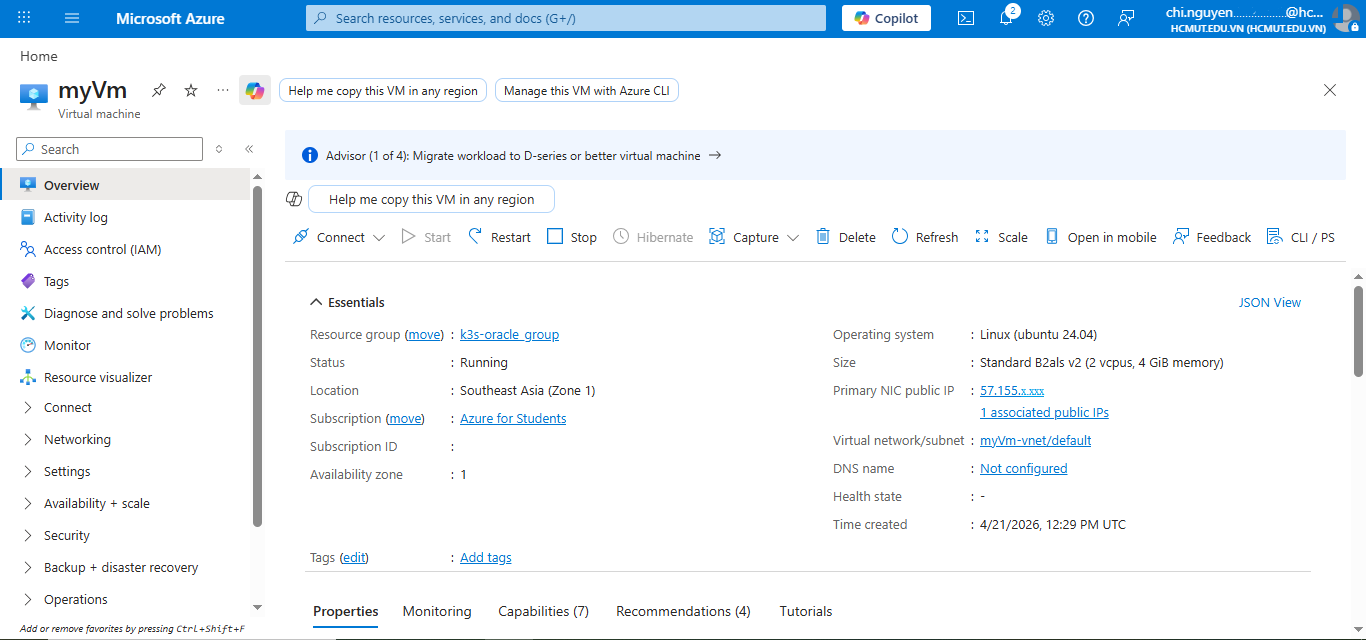
\includegraphics[width=0.9\textwidth]{images/chap7/backend/azure_machine.PNG}
    \vspace{0.7 cm}
    \caption{Giao diện quản lý Virtual Machine (myVm) trên Microsoft Azure Portal}
    \label{fig:azure_vm}
\end{figure}

Hình \ref{fig:azure_vm} hiển thị trạng thái hoạt động của máy ảo được sử dụng để triển khai hệ thống Backend. Máy ảo thuộc dòng Standard B2als v2 với 2 vCPUs và 4 GiB Memory, chạy hệ điều hành Ubuntu 24.04 và được đặt tại khu vực Southeast Asia để đảm bảo độ trễ thấp nhất cho người dùng tại Việt Nam.

\textbf{Quy trình đóng gói và xây dựng Image} 

Quá trình triển khai được thực hiện theo quy trình thủ công nhằm kiểm soát chặt chẽ các phiên bản thực thi:

\begin{itemize}
    \item Các dịch vụ Backend được đóng gói thành file \texttt{.jar} tại máy cục bộ để đảm bảo tính ổn định của mã nguồn sau khi kiểm thử.
    \item File \texttt{.jar} cùng với Dockerfile được chuyển lên máy ảo Azure thông qua giao thức bảo mật.
    \item Tại máy ảo, lệnh \texttt{docker build} được thực thi để tạo các Docker Image. Các Image này sử dụng cơ chế Multi-stage build với môi trường JRE nhẹ để tối ưu hóa dung lượng lưu trữ trên ổ đĩa của máy ảo.
\end{itemize}

Hình \ref{fig:docker_build} minh họa quá trình đóng gói thực tế, trong đó các lớp của image được xây dựng dựa trên Dockerfile đã thiết kế, đảm bảo môi trường vận hành được cô lập hoàn toàn.

\begin{figure}[H]
    \centering
    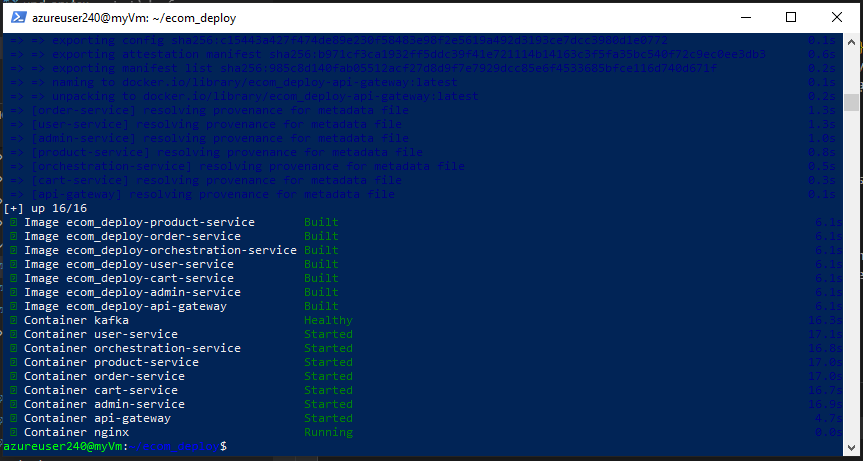
\includegraphics[width=0.9\textwidth]{images/chap7/backend/vm_running.PNG} 
    \vspace{0.7cm}
    \caption{Quá trình thực thi lệnh docker build để đóng gói dịch vụ trên máy ảo Azure}
    \label{fig:docker_build}
\end{figure}

\textbf{Điều phối hệ thống với Docker Compose}

Hệ thống sử dụng Docker Compose trên máy ảo để quản lý vòng đời và sự kết nối giữa các container:

\begin{itemize}
    \item \textbf{API Gateway Service:} API Gateway được triển khai như một dịch vụ độc lập bên trong mạng lưới microservices. Đây là thành phần duy nhất được cấu hình mở cổng kết nối thông qua Azure Network Security Group (NSG) để tiếp nhận và điều phối các yêu cầu từ Client vào hệ thống.
    \item \textbf{Quản lý hạ tầng:} Docker Compose điều phối các container PostgreSQL, Kafka và Zookeeper, thiết lập các Docker Volume để đảm bảo dữ liệu không bị mất khi container khởi động lại.
    \item \textbf{Mạng nội bộ (Virtual Network):} Tất cả các service giao tiếp với nhau trong một mạng nội bộ ảo của Docker. Các dịch vụ nghiệp vụ được ẩn hoàn toàn khỏi Internet, chỉ có thể truy cập thông qua luồng điều phối của API Gateway Service, giúp tăng cường bảo mật cho toàn hệ thống.
\end{itemize}

